\documentclass{article}
\usepackage[T1]{fontenc}
\usepackage{lmodern}
\usepackage{graphicx}
\usepackage{amsmath,amssymb}
\usepackage[a4paper,margin=2cm]{geometry}
\usepackage[absolute,overlay]{textpos}
\setlength{\TPHorizModule}{1mm}
\setlength{\TPVertModule}{1mm}
\usepackage[indonesian]{babel}
\usepackage{hyperref}
\setlength{\emergencystretch}{2em}
% unit: Halaman 15

\begin{document}

% === Halaman 15 (llm) ===

\vspace{239.98mm}

Demo Caesar Cipher Online: https://cryptii.com/pipes/caesar-cipher\vspace{10mm}

% deskripsi: Screenshot antarmuka situs web Cryptii yang menunjukkan proses enkripsi teks 'The quick brown fox jumps over the lazy dog' menggunakan Caesar cipher dengan shift 8, menghasilkan ciphertext 'Bpm ycqks ycqks jzvw nwf rcuxa wdmz bpm tihg lwo'.
% bbox normalisasi: [0.7700, 0.1340, 0.9020, 0.9420]
\begin{textblock*}{27.72mm}(161.70mm,39.80mm)
\noindent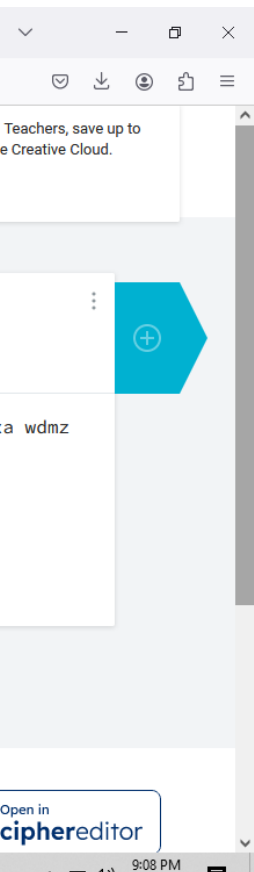
\includegraphics[width=27.72mm,height=239.98mm]{../../images/llm/page_015_img_01.png}%
\end{textblock*}

\end{document}
